\documentclass[border=15pt, multi, tikz]{standalone}
\usepackage{pgfplots}
\usepackage{import}
\usepackage{etoolbox}
\usepackage{graphicx}
\usepackage{svg}
\usepackage{colortbl}

\usetikzlibrary{positioning,matrix,fit}
\usetikzlibrary{3d} %for including external image
\usetikzlibrary{decorations,shapes}
\usetikzlibrary{decorations.shapes}
\usetikzlibrary{decorations.markings}
\usetikzlibrary{decorations.pathreplacing}
\usetikzlibrary{backgrounds}
\usetikzlibrary{calc}
\usetikzlibrary{arrows.meta,arrows}
\graphicspath{{image/}}
\usepackage{bm}
\usepackage{relsize}


\begin{document}
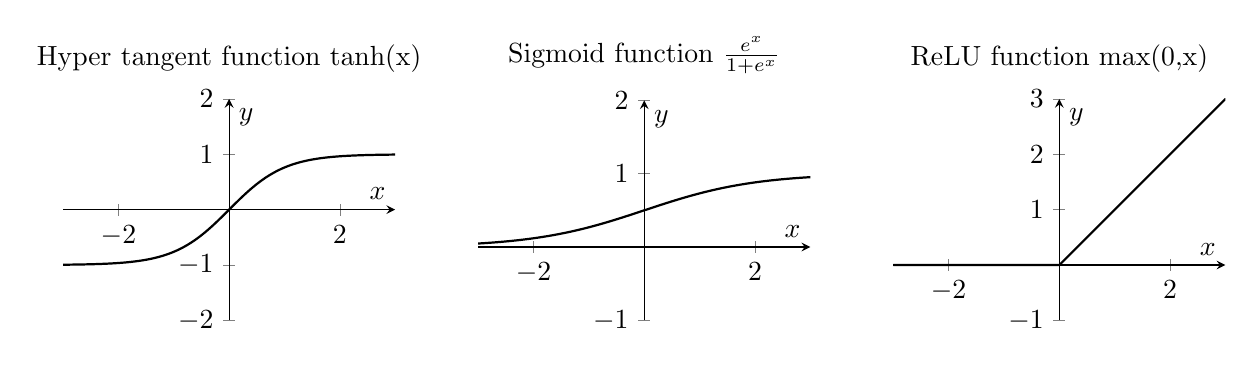
\begin{tikzpicture}
\begin{axis}[
            title = Hyper tangent function tanh(x),
            axis lines =center,
            xlabel = $x$, ylabel =$y$,
			samples=1000, domain=-4:4,
				xmin=-3, xmax=3,
				ymin=-2, ymax=2,
		        x=20, y=20,
				trig format = rad
			]
			\addplot expression [no markers, smooth, thick, black] {tanh(\x)};
			
\end{axis}
\begin{axis}[xshift=150,
            title = Sigmoid function $\frac{e^x}{1+e^x}$,
            axis lines =center,
            xlabel = $x$, ylabel =$y$, 
			samples=1000, domain=-4:4,
				x=10, y=10,
				xmin=-3, xmax=3,
				ymin=-1, ymax=2,
			    trig format = rad,
			    x=20, y=26.5,
			]
			\addplot expression [no markers, smooth, thick, black] {e^\x/(1+e^\x)};
\end{axis}
\begin{axis}[xshift=300,
            title = {{ReLU function max(0,x)}},
            axis lines =center,
            xlabel = $x$, ylabel =$y$, 
			samples=1000, domain=-4:4,
				x=10, y=10,
				xmin=-3, xmax=3,
				ymin=-1, ymax=3,
			    trig format = rad,
			    x=20, y=20,
			]
			\addplot expression [no markers, smooth, thick, black] {max(0,\x)};
\end{axis}
\end{tikzpicture}
\end{document}